\section{Auftrieb und Strömungswiderstand}

Dieser Versuch soll die Funktionsweise einer Tragfläche demonstrieren und auch den Einfluss des Anstellwinkels auf den Auftrieb (Kraft nach oben) und Rücktrieb aufzeigen. Mit diesen Werten sollen der beste Anstellwinkel der Tragfläche gefunden werden, was durch das Verhältnis von Auftriebs- und Widerstandskraft ausgedrückt wird. Da dieser Term gleichzeitig bei einem Gleitflug das Verhältnis von zurückgelegter Wegstrecke und Höhenverlust darstellt und somit ein guter Indikator für den besten Anstellwinkel der Tragfläche ist (manchmal wird die Gleitzahl auch als Kerhwert der hier genannten Größe definiert, für dieses Protokoll wird aber die genannte Definition verwendet).

\subsection{Messaufbau}

Die Tragfläche wird an einer Auftriebswaage befestig, wobei gleichzeitig durch einen Kraftmesser der Rücktrieb gemessen werden kann. Dann wird mit einer konstante Windgeschwindigkeit von \SI{14.38}{\metre\per\second} und für verschieden Anstellwinkel der Tragfläche der Auftrieb und der Rücktrieb gemessen.

\subsection{Auswertung}

Wie man in den Abbildungen \ref{fig:Aeoromechanik Versuch 3.11} und \ref{fig:Aeromechanik Versuch 3.12} erkennen kann steigt der Aufrieb stetig mit dem Anstellwinkel, wobei der Rücktrieb bei den gemessenene Werten ein Minimum bei einem Anstellwinkel von 10 Grad hat. Um nun den besten Kompromiss aus den beiden zu finden, also eine möglichst großen Auftrieb bei möglichst kleinem Rücktrieb, wird ein Polarendiagramm angefertigt siehe Abbildung \ref{fig:Aeromechanik Versuch 3.13}. Um nun den besten besten Anstellwinkel zu finden, werden Gerade durhc die Datenpunkte gelegt und die Gerade mit der größten Steigung gewählt (In unserem Fall also die blaue Gerade). Die Gleitzahl ergibt sich nun aus dem Verhältnis von Auftrieb und Rücktrieb, wir erhalten also:  $Gleitzahl \approx 2.35$. Somit ergibt sich bei einem Anstellwinkel von 10 Grad die größtmögliche Gleitdistanz bei kleinstem Höhenverlust im Gleitflug.

\begin{itemize}
    \item Erhöhung der Wölbung des Tragflügels
    \item Glättung der Oberfläche der Tragfläche
    \item Anbringen von Winglets (weniger Strömungswiderstand)
    \item Anbringen von Auftriebshilfen z.B. Krügerklappe (Kippnase)
\end{itemize}

\begin{figure}
    \centering
    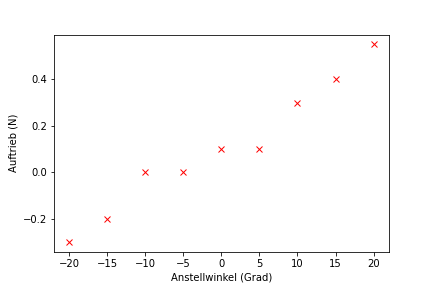
\includegraphics[scale=0.8]{Aeromechanik/Protokoll/fig/Aeromechanik Versuch 3.11.png}
    \caption{Verhältnis von Auftrieb und Anstellwinkel bei konstanter Windgeschwindigkeit}
    \label{fig:Aeoromechanik Versuch 3.11}
\end{figure}

\begin{figure}
    \centering
    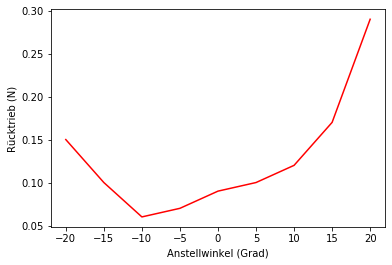
\includegraphics[scale=0.8]{Aeromechanik/Protokoll/fig/Aeromechanik Versuch 3.12.png}
    \caption{Verhältnis von Rücktrieb und Anstellwinkel bei konstanter Windgeschwindigkeit}
    \label{fig:Aeromechanik Versuch 3.12}
\end{figure}

\begin{figure}
    \centering
    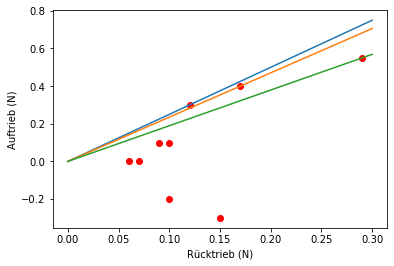
\includegraphics[scale=0.8]{Aeromechanik/Protokoll/fig/Aeromechanik Versuch 3.13.png}
    \caption{Verhältnis von Auftrieb und Rücktrieb bei konstanter Windgeschwindigkeit um die größte Gleitzahl zu finden}
    \label{fig:Aeromechanik Versuch 3.13}
\end{figure}

\section{Druckmessung}

\begin{figure}[h!]
    \centering
    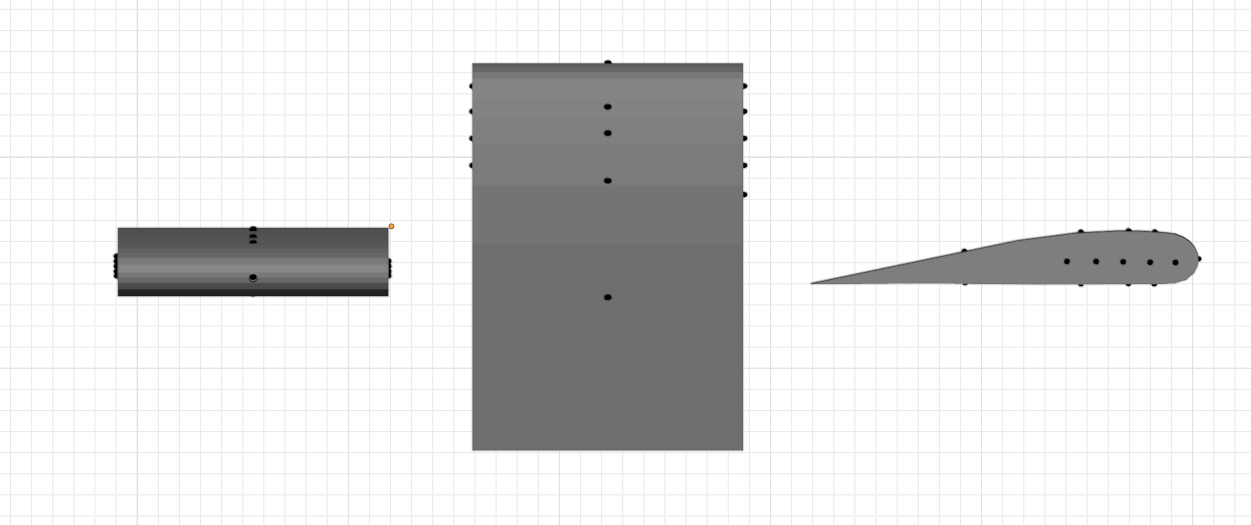
\includegraphics[scale=0.5]{./Aeromechanik/Protokoll/fig/lochpos.png}
    \caption{Lochpositionen am Flügel}
    \label{fig:Venturi}
\end{figure}

Im letzten Versuchsteil wird an neun verschiedenen Stellen der Druck an der Tragfläche gemessen. Die in Tabelle \ref{tab:Aeromechanik Versuch 3.2} aufgetragenen Werte, werden in einer Skizze als Druckvektoren visualisiert um den vorherschenden Druck besser einzuordnen. Dabei sind diese Vektoren zueinander normiert, wobei ein Pfeil nach innen einen positiven Druck und ein Pfeil vom Flügel weg einen negativen Druck bedeutet.

\begin{figure}[h!]
    \centering
    \includegraphics[scale=0.5]{./Aeromechanik/Protokoll/fig/Flügel_Vektor.png}
    \caption{Druckvektoren am Flügel bei verschiedenen Winkelstellungen}
    \label{fig:Venturi}
\end{figure}

\begin{table}
    \centering
    \caption{Druck für drei verschiedene Anstellwinkel, bei neun verschiedenen Messstellen (alle Messwerte in Pascal)}
    \begin{tabular}{c c c c}
    \hline
    Messstelle & 0 Grad & -20 Grad & 20 Grad \\
    \hline
    1 & 105 & 77 & 57 \\
    2 & -35 &  28 & -66 \\
    3 & -30 & -6 & -35 \\
    4 & -11 & -11 & -8 \\
    5 & -5 & -7 & -3 \\
    6 & -40 & -5 & 31 \\
    7 & -8 & -6 & 20 \\
    8 & 0 & -5 & 6 \\
    9 & 0 & -2 & 4 \\
    \hline
    \end{tabular}
    \label{tab:Aeromechanik Versuch 3.2}
\end{table}

In der Skizze kann man gut das Funktionsprinzip einer Tragfläche erkennen. Durch die Wölbung der Oberseite der Tragfläche entsteht dort ein Unterdruck relativ zur Unterseite des Flügels, durch diese Druckdifferenz wird die Tragfläche und somit auch das Flugzeug nach oben gedrückt. Mit den Ergebnissen aus der vorherigen Aufgabe, lässt sich die Schwierigkeit eines perfekten Tragflächenprofils zeigen, da die Ingenieure einen für den Anwendungszweck optimierten Mittelweg zwischen rücktriebender Kraft und Auftrieb finden müssen. Um nun noch einen einstellbaren Auftrieb bei konstanter Geschwindigkeit möglich zu machen, könnte man den Flügel, wie durch Grafik \ref{fig:Aeromechanik Versuch 3.13} gezeigt, drehen, um den gewünschten Auftrieb zu erhalten. Allerdings wird bei modernen Flugzeugen auf eine modulare Tragprofilform gesetzt, die es durch Quer- und Höhenruder erlaubt, den gewünschten Auftrieb zu erreichen, was gerade beim Start und Landen von Flugzeugen von enormer Bedeutung ist.

